% Options for packages loaded elsewhere
\PassOptionsToPackage{unicode}{hyperref}
\PassOptionsToPackage{hyphens}{url}
\PassOptionsToPackage{dvipsnames,svgnames,x11names}{xcolor}
%
\documentclass[
  letterpaper,
  DIV=11,
  numbers=noendperiod]{scrartcl}

\usepackage{amsmath,amssymb}
\usepackage{lmodern}
\usepackage{iftex}
\ifPDFTeX
  \usepackage[T1]{fontenc}
  \usepackage[utf8]{inputenc}
  \usepackage{textcomp} % provide euro and other symbols
\else % if luatex or xetex
  \usepackage{unicode-math}
  \defaultfontfeatures{Scale=MatchLowercase}
  \defaultfontfeatures[\rmfamily]{Ligatures=TeX,Scale=1}
\fi
% Use upquote if available, for straight quotes in verbatim environments
\IfFileExists{upquote.sty}{\usepackage{upquote}}{}
\IfFileExists{microtype.sty}{% use microtype if available
  \usepackage[]{microtype}
  \UseMicrotypeSet[protrusion]{basicmath} % disable protrusion for tt fonts
}{}
\makeatletter
\@ifundefined{KOMAClassName}{% if non-KOMA class
  \IfFileExists{parskip.sty}{%
    \usepackage{parskip}
  }{% else
    \setlength{\parindent}{0pt}
    \setlength{\parskip}{6pt plus 2pt minus 1pt}}
}{% if KOMA class
  \KOMAoptions{parskip=half}}
\makeatother
\usepackage{xcolor}
\setlength{\emergencystretch}{3em} % prevent overfull lines
\setcounter{secnumdepth}{-\maxdimen} % remove section numbering
% Make \paragraph and \subparagraph free-standing
\ifx\paragraph\undefined\else
  \let\oldparagraph\paragraph
  \renewcommand{\paragraph}[1]{\oldparagraph{#1}\mbox{}}
\fi
\ifx\subparagraph\undefined\else
  \let\oldsubparagraph\subparagraph
  \renewcommand{\subparagraph}[1]{\oldsubparagraph{#1}\mbox{}}
\fi


\providecommand{\tightlist}{%
  \setlength{\itemsep}{0pt}\setlength{\parskip}{0pt}}\usepackage{longtable,booktabs,array}
\usepackage{calc} % for calculating minipage widths
% Correct order of tables after \paragraph or \subparagraph
\usepackage{etoolbox}
\makeatletter
\patchcmd\longtable{\par}{\if@noskipsec\mbox{}\fi\par}{}{}
\makeatother
% Allow footnotes in longtable head/foot
\IfFileExists{footnotehyper.sty}{\usepackage{footnotehyper}}{\usepackage{footnote}}
\makesavenoteenv{longtable}
\usepackage{graphicx}
\makeatletter
\def\maxwidth{\ifdim\Gin@nat@width>\linewidth\linewidth\else\Gin@nat@width\fi}
\def\maxheight{\ifdim\Gin@nat@height>\textheight\textheight\else\Gin@nat@height\fi}
\makeatother
% Scale images if necessary, so that they will not overflow the page
% margins by default, and it is still possible to overwrite the defaults
% using explicit options in \includegraphics[width, height, ...]{}
\setkeys{Gin}{width=\maxwidth,height=\maxheight,keepaspectratio}
% Set default figure placement to htbp
\makeatletter
\def\fps@figure{htbp}
\makeatother

\usepackage{booktabs}
\usepackage{longtable}
\usepackage{array}
\usepackage{multirow}
\usepackage{wrapfig}
\usepackage{float}
\usepackage{colortbl}
\usepackage{pdflscape}
\usepackage{tabu}
\usepackage{threeparttable}
\usepackage{threeparttablex}
\usepackage[normalem]{ulem}
\usepackage{makecell}
\usepackage{xcolor}
\KOMAoption{captions}{tableheading}
\makeatletter
\makeatother
\makeatletter
\makeatother
\makeatletter
\@ifpackageloaded{caption}{}{\usepackage{caption}}
\AtBeginDocument{%
\ifdefined\contentsname
  \renewcommand*\contentsname{Table of contents}
\else
  \newcommand\contentsname{Table of contents}
\fi
\ifdefined\listfigurename
  \renewcommand*\listfigurename{List of Figures}
\else
  \newcommand\listfigurename{List of Figures}
\fi
\ifdefined\listtablename
  \renewcommand*\listtablename{List of Tables}
\else
  \newcommand\listtablename{List of Tables}
\fi
\ifdefined\figurename
  \renewcommand*\figurename{Figure}
\else
  \newcommand\figurename{Figure}
\fi
\ifdefined\tablename
  \renewcommand*\tablename{Table}
\else
  \newcommand\tablename{Table}
\fi
}
\@ifpackageloaded{float}{}{\usepackage{float}}
\floatstyle{ruled}
\@ifundefined{c@chapter}{\newfloat{codelisting}{h}{lop}}{\newfloat{codelisting}{h}{lop}[chapter]}
\floatname{codelisting}{Listing}
\newcommand*\listoflistings{\listof{codelisting}{List of Listings}}
\makeatother
\makeatletter
\@ifpackageloaded{caption}{}{\usepackage{caption}}
\@ifpackageloaded{subcaption}{}{\usepackage{subcaption}}
\makeatother
\makeatletter
\@ifpackageloaded{tcolorbox}{}{\usepackage[many]{tcolorbox}}
\makeatother
\makeatletter
\@ifundefined{shadecolor}{\definecolor{shadecolor}{rgb}{.97, .97, .97}}
\makeatother
\makeatletter
\makeatother
\ifLuaTeX
  \usepackage{selnolig}  % disable illegal ligatures
\fi
\IfFileExists{bookmark.sty}{\usepackage{bookmark}}{\usepackage{hyperref}}
\IfFileExists{xurl.sty}{\usepackage{xurl}}{} % add URL line breaks if available
\urlstyle{same} % disable monospaced font for URLs
\hypersetup{
  pdftitle={Palmer penguins},
  pdfauthor={Athanasia Mo Mowinckel},
  colorlinks=true,
  linkcolor={blue},
  filecolor={Maroon},
  citecolor={Blue},
  urlcolor={Blue},
  pdfcreator={LaTeX via pandoc}}

\title{Palmer penguins}
\author{Athanasia Mo Mowinckel}
\date{10/26/22}

\begin{document}
\maketitle
\ifdefined\Shaded\renewenvironment{Shaded}{\begin{tcolorbox}[interior hidden, borderline west={3pt}{0pt}{shadecolor}, breakable, frame hidden, boxrule=0pt, enhanced, sharp corners]}{\end{tcolorbox}}\fi

\renewcommand*\contentsname{Contents}
{
\hypersetup{linkcolor=}
\setcounter{tocdepth}{2}
\tableofcontents
}
\hfill\break
We can write text as normal, interspersed with code that outputs
something. We can choose to have the code shown or hidden, or provide
the reader with the option to see the code if they wish.

My favourite foods:

\begin{enumerate}
\def\labelenumi{\arabic{enumi}.}
\tightlist
\item
  Souvlaki
\item
  Pasta with halloumi
\item
  Makaronia tou fournou (greek style lasagna)
\end{enumerate}

We can also reference the figures Figure~\ref{fig-penguin-smooth} and
Figure~\ref{fig-penguin-density}

\begin{figure}

{\centering 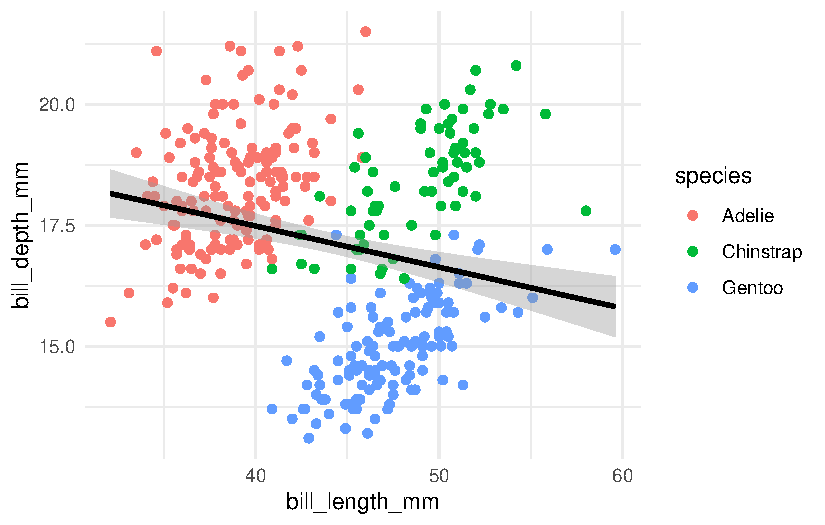
\includegraphics{03_pdf_example_files/figure-pdf/fig-penguin-smooth-1.pdf}

}

\caption{\label{fig-penguin-smooth}Penguin bill length and depth ratio
by species}

\end{figure}

And the order of the figures does not really matter. If you change the
order to the figures, but keep their labels, no references will be
broken in the report. We can also incorporate text derived from data to
look as if it were ``normal'' text. Like the number of rows in the data
being 344, and the number of female penguins being 165. We can also add
footnotes\footnote{which can be very convenient}, and they will keep
themselves numbered and placed correctly\footnote{without us really
  needing to keep it all in mind.}

\begin{figure}

{\centering 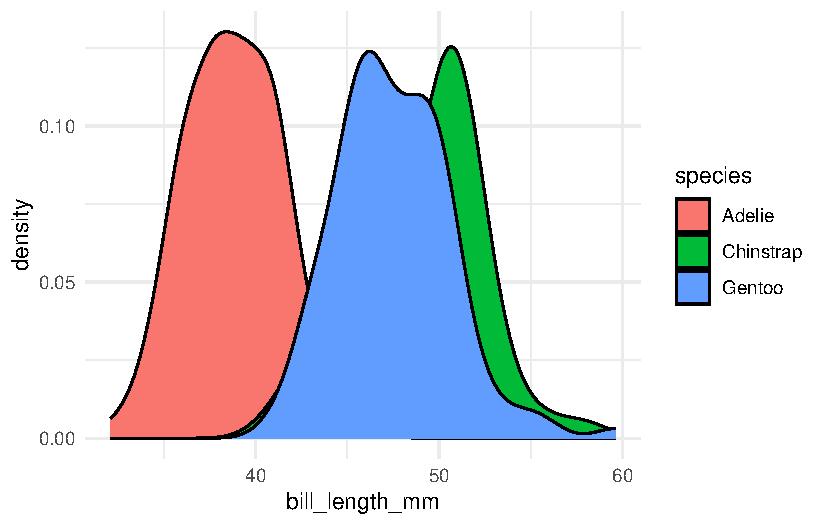
\includegraphics{03_pdf_example_files/figure-pdf/fig-penguin-density-1.pdf}

}

\caption{\label{fig-penguin-density}Penguin density}

\end{figure}

A summary of the observed penguin data can be found in
Table~\ref{tbl-penguins}. For this cross-reference to work, we
\emph{need} to have the \texttt{tbl-} prefix in the label name of the
chunk that creates the table. The number of the table will update if
another table appears before it, meaning you no longer need to deal with
number your content correctly.\\

\hypertarget{tbl-penguins}{}
\begin{table}
\caption{\label{tbl-penguins}Penguin summary }\tabularnewline

\centering
\begin{tabular}{llrrrrr}
\toprule
\multicolumn{4}{c}{ } & \multicolumn{2}{c}{Range} & \multicolumn{1}{c}{ } \\
\cmidrule(l{3pt}r{3pt}){5-6}
name & species & Mean & SD & Min & Max & N\\
\midrule
 & Adelie & 18.346 & 1.217 & 15.5 & 21.5 & 151\\
\cmidrule{2-7}
 & Chinstrap & 18.421 & 1.135 & 16.4 & 20.8 & 68\\
\cmidrule{2-7}
\multirow{-3}{*}{\raggedright\arraybackslash bill depth mm} & Gentoo & 14.982 & 0.981 & 13.1 & 17.3 & 123\\
\cmidrule{1-7}
 & Adelie & 38.791 & 2.663 & 32.1 & 46.0 & 151\\
\cmidrule{2-7}
 & Chinstrap & 48.834 & 3.339 & 40.9 & 58.0 & 68\\
\cmidrule{2-7}
\multirow{-3}{*}{\raggedright\arraybackslash bill length mm} & Gentoo & 47.505 & 3.082 & 40.9 & 59.6 & 123\\
\cmidrule{1-7}
 & Adelie & 3700.662 & 458.566 & 2850.0 & 4775.0 & 151\\
\cmidrule{2-7}
 & Chinstrap & 3733.088 & 384.335 & 2700.0 & 4800.0 & 68\\
\cmidrule{2-7}
\multirow{-3}{*}{\raggedright\arraybackslash body mass g} & Gentoo & 5076.016 & 504.116 & 3950.0 & 6300.0 & 123\\
\cmidrule{1-7}
 & Adelie & 189.954 & 6.539 & 172.0 & 210.0 & 151\\
\cmidrule{2-7}
 & Chinstrap & 195.824 & 7.132 & 178.0 & 212.0 & 68\\
\cmidrule{2-7}
\multirow{-3}{*}{\raggedright\arraybackslash flipper length mm} & Gentoo & 217.187 & 6.485 & 203.0 & 231.0 & 123\\
\bottomrule
\end{tabular}
\end{table}



\end{document}
